% Figure 20 -- (a) 3d mirror for rank N A_1 theory, (b) for rank N A_2 theory
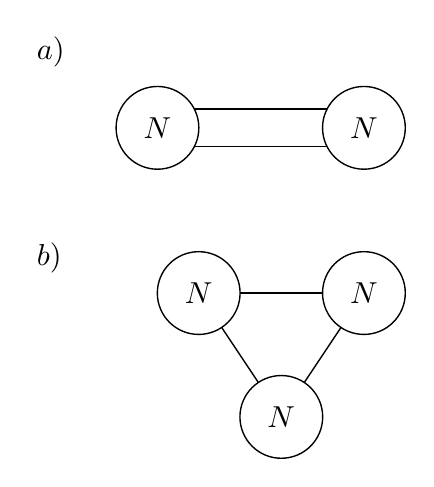
\begin{tikzpicture}[x=1pt,y=1pt,>=stealth,line width=0.5pt,
   nd/.style={circle,draw,fill=white,minimum size=29.9pt,inner sep=0pt,
              font=\fontsize{11}{11}\selectfont}]
  % ---------------- a) ----------------
  \draw (59.15,140.1) -- (133.75,140.1);
  \draw (59.15,126.6) -- (133.75,126.6);
  \node[nd] at (59.15,133.35) {$N$};
  \node[nd] at (133.75,133.35) {$N$};
  \node[anchor=base west,font=\fontsize{10.7}{10.7}\selectfont] at (12,158) {$a)$};
  % ---------------- b) ----------------
  \draw (74.05,73.65) -- (133.75,73.65);
  \draw (74.05,73.65) -- (103.9,28.9);
  \draw (133.75,73.65) -- (103.9,28.9);
  \node[nd] at (74.05,73.65) {$N$};
  \node[nd] at (133.75,73.65) {$N$};
  \node[nd] at (103.9,28.9) {$N$};
  \node[anchor=base west,font=\fontsize{10.7}{10.7}\selectfont] at (12,83.5) {$b)$};
\end{tikzpicture}
